\documentclass{beamer}
\usepackage[british]{babel}
\usepackage[utf8]{inputenc}
\usepackage{graphicx,hyperref,ucr_eie,url}
\usepackage{mdframed}
\usepackage{tikz}
\usetikzlibrary{snakes}
\usepackage{chronology}
\usepackage{listings}
\graphicspath{{../multimedia/images/}}
\definecolor{shadecolor}{RGB}{250,250,250}		%%boxes color
\lstset{
		basicstyle=\ttfamily,
		keywordstyle=\color{black},
		commentstyle=\color{black},
		stringstyle=\color{black},
		tabsize=2,
		backgroundcolor=\color{shadecolor}}

% The title of the presentation:
%  - first a short version which is visible at the bottom of each slide;
%  - second the full title shown on the title slide;
\title[Use of OpenCV to Send Commands]{7} 

% Optional: a subtitle to be dispalyed on the title slide
%\subtitle{}

% The author(s) of the presentation:
%  - again first a short version to be displayed at the bottom;
%  - next the full list of authors, which may include contact information;
\author[Jose Pablo Apú - B10407]{
  Francisco Mata\\
  Jose Pablo Apú Picado\\
  Sebastian Ramírez Solano\\\medskip
  %{\small \url{p.vullers@cs.ru.nl}} \\ 
  %{\small \url{http://www.cs.ru.nl/~pim/}}}
  }

% The institute:
%  - to start the name of the university as displayed on the top of each slide
%    this can be adjusted such that you can also create a Dutch version
%  - next the institute information as displayed on the title slide
\institute[University of Costa Rica]{
  Electrical Engineering School \\
  IE-0117 - Programación Bajo Plataformas Abiertas}

% Add a date and possibly the name of the event to the slides
%  - again first a short version to be shown at the bottom of each slide
%  - second the full date and event name for the title slide
\date[\today]{
  2nd Development Project \\
  \today}

\begin{document}

\begin{frame}
  \titlepage
\end{frame}

\begin{frame}
  \frametitle{Outline}
  \tableofcontents
\end{frame}

% Section titles are shown in at the top of the slides with the current section 
% highlighted. Note that the number of sections determines the size of the top 
% bar, and hence the university name and logo. If you do not add any sections 
% they will not be visible.
%%*****************************************************************************
\section{Introduction}

\begin{frame}
\frametitle{Objectives}

\end{frame}
%%*****************************************************************************
\begin{frame}
\frametitle{Justification}

\end{frame}
%%*****************************************************************************
\section{Requirements}

\begin{frame}
\frametitle{Hardware}
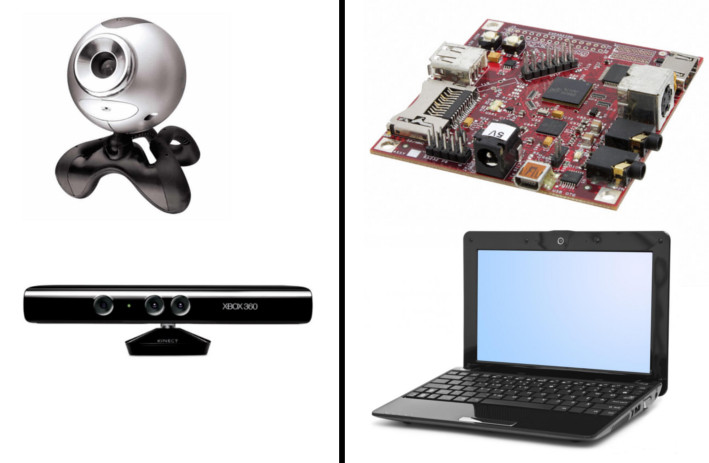
\includegraphics[scale=0.4]{requirements_hardware.jpg}
\end{frame}
%%*****************************************************************************
\begin{frame}
\frametitle{Software}
\begin{center}
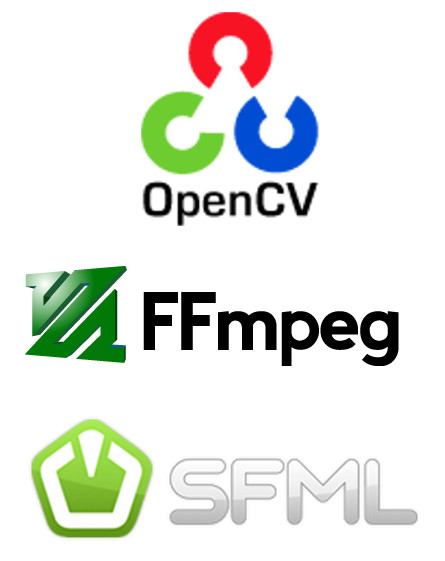
\includegraphics[scale=0.3]{requirements_libs.jpg}
\end{center}
\end{frame}
%%*****************************************************************************
\section{Computer Vision}

\begin{frame}
\frametitle{Main concepts}
\end{frame}
%%*****************************************************************************
\begin{frame}
\frametitle{Typical tasks of computer vision}

\end{frame}
%%*****************************************************************************
\section{Why the use of a database?}
\begin{frame}
\frametitle{}
\end{frame}
%%*****************************************************************************
\begin{frame}
\frametitle{}
\end{frame}
%%*****************************************************************************
\begin{frame}
\frametitle{Perl Basics - Fields of Application}

\end{frame}
%%*****************************************************************************
\begin{frame}
\frametitle{}
\end{frame}
%%*****************************************************************************
\begin{frame}
\frametitle{}
\end{frame}
%%*****************************************************************************
\section{Source Code}
\begin{frame}[fragile]
\frametitle{Programming Interface - Example}
\begin{lstlisting}
#!/usr/bin/perl

open(GRADES, "grades") or die "Error: $!\n";

while ($line = <GRADES>) {
($student, $grade) = split(" ", $line);
$grades{$student} .= $grade . " ";
}

foreach $student (sort keys %grades) {
$scores = 0;
$total = 0;
@grades = split(" ", $grades{$student});
\end{lstlisting}
\end{frame}
%%*****************************************************************************
\begin{frame}[fragile]
\frametitle{Programming Interface - Example}
\begin{lstlisting}
foreach $grade (@grades) {
$total += $grade;
$scores++;
}
$average = $total / $scores;
print "$student: $grades{$student}"
print "\t\tAverage: $average\n";
}
\end{lstlisting}
\end{frame}
%%*****************************************************************************
\begin{frame}[fragile]
\frametitle{Programming Interface - Example}
\end{frame}
%%*****************************************************************************
\section{Conclusion}
\begin{frame}
 \frametitle{Conclusion}
\begin{itemize}
\item Excelent for Text Processing
\item It is Pearl better than the other ones?
%\item Documentation
\end{itemize}
%Moose
%fork
\end{frame}
%%*****************************************************************************
\begin{frame}
 \frametitle{Questions?}
\end{frame}
%%*****************************************************************************
\begin{frame}
 \frametitle{Reference - Books}
\begin{thebibliography}{10}
\bibitem{label}Marco, M. Marco, J (2010) Escanenado la Infomática. Editorial UOC. 
%%http://books.google.co.cr/books?id=svpzjkMpdiUC&pg=PA124&dq=paradigmas+programacion&hl=es-419&sa=X&ei=v2WWUbyANqLn0wHi-oDACA&redir_esc=y#v=onepage&q=paradigmas%20programacion&f=false}
\bibitem{pascal}Berlanfa, R., García, P. 2000 Introdución a la programación con PASCAL Universidad Jaiume I, ed. III.
%%http://books.google.co.cr/books?id=OZFmZfOkz94C&pg=PA49&dq=lenguaje+Pascal&hl=es-419&sa=X&ei=TuiaUa6mIs-30AHVm4CAAg&redir_esc=y#v=onepage&q=lenguaje%20Pascal&f=false
\bibitem{actionscript}Curso de Flash CS4, aulaClic S.L.
%%http://books.google.co.cr/books?id=86mUhf-GiEYC&dq=lenguaje+ActionScript&source=gbs_navlinks_s
\end{thebibliography}
\end{frame}

\begin{frame}
 \frametitle{Reference - PDF's}
\begin{thebibliography}{10}
\bibitem{pearl}PEARL 90 - Language Report, 1998
%%http://www.irt.uni-hannover.de/pearl/pub/report.pdf
\bibitem{ruby}Guía de usuario de Ruby
%%http://www.google.com/url?sa=t&rct=j&q=&esrc=s&source=web&cd=1&ved=0CDEQFjAA&url=http%3A%2F%2Fes.tldp.org%2FManuales-LuCAS%2Fdoc-guia-usuario-ruby%2Fguia-usuario-ruby.pdf&ei=tuqaUeqfFeff0gH5m4GYDw&usg=AFQjCNG_rpdTQi6bymCwcQitvcwtcWHBAw&sig2=N-OTxrSSk4_WwGPt1vhUkA&bvm=bv.46751780,d.dmQ
\bibitem{simula}El Lenguaje Simula, creado por Fco Jesús Fdez Burgos.
%%http://www.google.com/url?sa=t&rct=j&q=&esrc=s&source=web&cd=2&ved=0CDkQFjAB&url=http%3A%2F%2Fwww.lcc.uma.es%2F~blas%2Fapuntes%2FPDAv%2Fp2005-2006%2FSIMULA1.pdf&ei=JeuaUYidKKXE0AGUkYCADw&usg=AFQjCNF9Vv6xinkTVBsM5RKrbIF7AUezJQ&sig2=S9c02kO0rJJfp5VCiwRNjQ&bvm=bv.46751780,d.dmQ
\bibitem{miranda}An overview of Miranda, creado por David Turner. 1986
%%http://www.google.com/url?sa=t&rct=j&q=&esrc=s&source=web&cd=1&ved=0CDAQFjAA&url=http%3A%2F%2Fwww.cs.kent.ac.uk%2Fpeople%2Fstaff%2Fdat%2Fmiranda%2Foverview.pdf&ei=peuaUamzHaaR0QGjg4HoAw&usg=AFQjCNGDycvrntqTcEOiHb4B70C92ibEDg&sig2=FeEanDC2s_tYTbdMh_2QDA&bvm=bv.46751780,d.dmQ
\bibitem{label}El Lenguaje Multi-paradigma.
%%http://www.google.com/url?sa=t&rct=j&q=&esrc=s&source=web&cd=1&ved=0CDEQFjAA&url=http%3A%2F%2Fwebs.uvigo.es%2Fjoselu%2Fmaterial%2FCurry_objetos.pdf&ei=YOyaUZnREJKP0QH78oGABw&usg=AFQjCNFxULggnO31OC1450LTpZFcFFdD2A&sig2=yPs7k7X5r0jHQctnA0tqoQ&bvm=bv.46751780,d.dmQ
\end{thebibliography}
\end{frame}

\begin{frame}
 \frametitle{Reference - PDF's}
\begin{thebibliography}{10}
\bibitem{pearl2}\url{http://houston.pm.org}
\bibitem{ruby2}\url{http://www.fincher.org/tips/Languages/Ruby/}
\bibitem{simula2} \url{http://staff.um.edu.mt/jskl1/talk.html}
\bibitem{miranda2} \url{http://miranda.org.uk/}
\bibitem{mathematica2}\url{http://www.wolfram.com/mathematica/}\end{thebibliography}
\end{frame}

\end{document}
